% !TEX root = main.tex

\chapter{Dosimetria}
La dosimetria e' una branca a cavallo tra la fisica e la medicina che definisce le grandezze fisiche che hanno la maggior probabilità di essere correlate a grandezze cliniche (quale la sopravvivenza dei pazienti). Questa quantificazione e' necessaria sia per esposizioni accidentali alla radiazioni, quali nel caso di incidenti nucleari, che per esposizioni intenzionali a radiazioni per fini terapeutici. Partiamo considerando alcuni ordini di grandezza:
Vi sono circa $10^{13}$ cellule nel corpo umano, ognuna con un diametro medio di $10 \ \mu m$, con un nucleo di $3 \ \mu m$ contenente DNA, che ha una larghezza tipica di $ 2 \ nm$ e la lunghezza di un gene è circa $0,1 \ \mu m$.  \\

Esistono due modi in cui una radiazione incidente può provocare la morte di una cellula, uno diretto ed uno indiretto. Per uccidere direttamente una cellula la radiazione incidente deve rompere legami in entrambe le eliche di un tratto del suo DNA in modo da renderlo difficilmente reparabile, perché nessuna delle due eliche potrà fare da stampo per la rigenerazione dell'elica complementare. \\
Ciò che accade più frequentemente però è che la cellula venga uccisa dalla radiazione incidente in modo indiretto. Questo avviene quando la radiazione ionizza le molecole d'acqua presenti nella cellula creando specie reattive come $\text{OH}^{-}$, $\text{O}_2^{-}$ e $\text{H}_2\text{O}_2$ che possono attaccare direttamente il DNA o portare alla sintetizzazione di altre sostanze analoghe a quelle adoperate nella chemioterapia che uccidono la cellula o ne inibiscono la riproduzione.\\
Gli effetti della radiazione possono essere distinti in stocastici o non-stocastici. Gli effetti stocastici sono quelli che sono privi di un livello di soglia di esposizione sotto il quale non vi sono effetti: ad ogni livello di esposizione dalla radiazione corrisponde una probabilità che si verifichino tali effetti, e la loro gravità non dipende dall'intensità della radiazione. Gli effetti non stocastici invece sono prevedibili ed avvengono oltre un certo livello di intensità di radiazione. La loro gravità inoltre dipende dall'intensità della radiazione.\\
Infine i danni da radiazione si possono dividere in somatici e genetici, a dipesa dal fatto che le cellule colpite siano quelle somatiche o quelle germinali.


\section{Grandezze Preliminari}

Si definiscono le seguenti grandezze:

\begin{itemize}
\item Fluenza $\phi=\frac{\mathrm{d}N}{\mathrm{d}A}$ è una proprietà strettamente della sorgente, come l'attività.
\item Flusso $\Phi=\frac{\mathrm{d}N}{\mathrm{d}A\mathrm{d}t}$
\item Fluenza di Energia $\psi=\frac{\mathrm{d}E}{\mathrm{d}A}$
\item Flusso di Energia $\Psi=\frac{\mathrm{d}E}{\mathrm{d}A\mathrm{d}t}$
\end{itemize}

\section{Esposizione}

L'esposizione, o exposure, è una grandezza esclusivamente legata alla radiazione neutra. \'E definita nel seguente modo:

\begin{equation}
X=\frac{\mathrm{d}q}{\mathrm{d}m}=\frac{1}{\rho}\frac{\mathrm{d}q}{\mathrm{d}V}
\end{equation}

Essa rappresenta la quantità di carica del mezzo che viene accelerata quando esso è investito da radiazione, per unità di massa. La sua unità di misura è la seguente:

\begin{equation}
1 Roentgen = 2,58 \times 10^{-4} \frac{C}{kg}
\end{equation}

C'è un modo indiretto di calcolarla. Se esprimo $\mathrm{d}q=\frac{eE_{\gamma}\mathrm{d}N }{w}$ dove $e$ è la carica dell'elettrone, $E_{\gamma}$ l'energia della radiazione neutra incidente, $\mathrm{d}N$ il numero di cariche accelerate e $w$ è l'energia di ionizzazione media (34 eV in aria), e se esprimo l'unità di massa come $\mathrm{d}m=\rho A \mathrm{d}x$, allora ho:

\begin{equation}
X=\frac{1}{\rho}\frac{e}{w}\frac{E_{\gamma}\mathrm{d}N}{A  \mathrm{d}x}=\frac{e  \mu  N E_{\gamma} }{ w  \rho A}=\frac{e \mu E_{\gamma} \phi}{w \rho}
\end{equation}

Dove si è tenuto conto del fatto che $\frac{N}{A}=\phi$ e che $\frac{\mathrm{d}N}{\mathrm{d}x}=\mu N$.

Spesso si parla di exposure rate, derivata nel tempo dell'exposure.

Nel caso specifico di sorgenti puntiformi di raggi $\gamma$ vale anche la seguente legge:

\begin{equation}
\frac{\mathrm{d}X}{\mathrm{d}t}=\Gamma\cdot\frac{A}{d^2}
\end{equation}

Dove $\Gamma$ è un coefficiente specifico di ogni sorgente, $A$ è l'attività di quella sorgente, $d$ è la distanza da tale sorgente.

\section{Dose}

La dose è definita come l'energia assorbita per radiazione dall'unità di massa del paziente:

\begin{equation}
D=\frac{\mathrm{d}E}{\mathrm{d}m}
\end{equation}

Essa è una proprietà collettiva dell'intero trattamento.

L'energia assorbita può essere esplicitata come segue

\begin{equation}
E=E_{rad_{i}}-E_{rad_{f}}+\sum \text{Q}
\end{equation}

Dove Q è il Q-value delle reazioni che avvengono nel caso considerato, che dunque può avere segno alterno in base al tipo di reazioni. Nel caso di irraggiamento da parte di un flusso di fotoni monocromatico vale la seguente uguaglianza:

\begin{equation}
\mathrm{d}E_{\gamma}=E_{\gamma}\mathrm{d}N
\end{equation}

Dunque la dose può essere espressa come segue:

\begin{equation}
D_{\gamma}=\frac{E_{\gamma}\mathrm{d}N}{\rho A\mathrm{d}x}=\frac{E_{\gamma}\mu N}{\rho A}=\frac{E_{\gamma}\mu \Phi}{\rho} 
\end{equation}

Dove si è tenuto in considerazione il fatto che $\mathrm{d}N/\mathrm{d}x=\mu N$ in modulo.\\

\textbf{E nel caso di un flusso di fotoni non monocromatico?}\\

Nel caso di irraggiamento da parte di un fascio di particelle cariche invece vale $\mathrm{d}E=N\mathrm{d}E$, dunque la dose viene espressa come segue:

\begin{equation}
D=\frac{N\mathrm{d}E}{\rho \mathrm{d}V}=\frac{N\mathrm{d}E}{\rho A \mathrm{d}x}=\frac{LET\cdot\phi}{\rho}
\end{equation}

In ogni caso l'unità di misura convenzionale è il Gray.

\begin{equation}
1 Gy = 1 \frac{J}{kg}
\end{equation}

\section{Confronto Tra Dose ed Esposizione}

Confrontando l'espressione della dose per i fotoni e l'esposizione, osserviamo che:

\begin{equation}
X=\frac{e}{w}\frac{\mu}{\rho}E_{\gamma}\phi=\frac{e}{w}D
\end{equation}

Ora, sapendo che $\frac{w_{aria}}{e}=8,74\cdot 10^{-3} \ Gy/R$ possiamo calcolare la dose in qualunque materiale conoscendo l'esposizione in aria di una certa radiazione, ricordando che $D_{aria}=X_{aria}\frac{w_{aria}}{e}$facendo come segue:

\begin{equation}
D_{m}=D_{aria}\frac{(\mu/\rho)_m}{(\mu/\rho)_{aria}}=X\frac{w_{aria}}{e}\frac{(\mu/\rho)_m}{(\mu/\rho)_{aria}}
\end{equation}



\section{Altre Grandezze di Dosimetria}

La radiazione incidente di cui possiamo calcolare la dose può essere più o meno dannosa per un certo tessuto. Per tenere conto di queste differenze si vuole esprimere con una grandezza unica la valutazione stocastica dei danni biologici che quella dose di radiazione in media farà su quel tessuto. Tale grandezza è la dose equivalente.

\begin{equation}
H=D\cdot Q
\end{equation}

Dove il fattore di proporzionalità Q è detto Quality Factor, e dipende dal tipo di radiazione incidente e dalla sua energia.
L'unità di misura della dose equivalente è la seguente:

\begin{equation}
1 Sv = 1 \frac{J}{kg}
\end{equation}

Essa corrisponde al Gray ma ha significato fisico evidentemente diverso.

La dose effettiva invece è la somma delle dosi equivalenti assorbite da ogni tessuto pesata con dei fattori che rappresentano la sensibilità di tale tessuto alla radiazione in considerazione.

\begin{equation}
E=\sum H_{T} W_{T}
\end{equation}

I parametri $W_{T}$ sono adimensionali, dunque l'unità di misura della dose effettiva rimane il Sievert.

Si definisce poi la Kinetic Energy Release in the Medium (KERMA), che come dice il nome è definita come segue:

\begin{equation}
\text{KERMA}=\frac{\Delta E_k}{\Delta m}
\end{equation}

Anche questa si misura in Gray. Corrisponde alla dose se $\Delta E_k$ è proprio la differenza tra energia entrante ed uscente da un volumetto.
Questa condizione è detta Charged Particle Equilibrium (CPE), e microscopicamente è verificata se ogni particella che porta via una certa energia dal volumetto è sostituita immediatamente da una particella identica che porta quella stessa energia nel volume. 
In generale mentre la dose è l'energia assorbita per unità di volume, la kerma è l'energia trasferita dalla particella o dal fotone originale in quella stessa unità di volume.

Si definisce poi la Relative Biological Effectiveness (RBE) come la
\begin{equation}
RBE=\frac{D(X)_{10\%}}{D(T)_{10\%}}
\end{equation}

Dove le due D sono le dosi rispettivamente di raggi X e della radiazione in esame necessarie ad avere un efficacia del 10\%. Più il parametro RBE è alto, più è buona la qualità del fascio.

\begin{figure} []
\centering
		%% 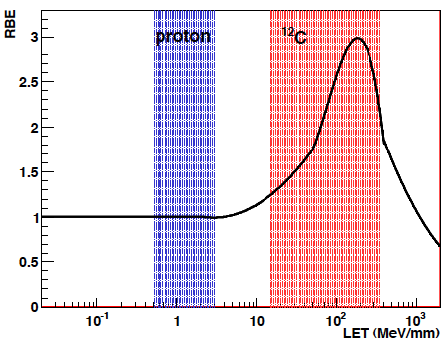
\includegraphics[width=8cm, keepaspectratio]{RBE.png}
		\caption{Relative Biological Effectiveness in funzione del LET}
         \label{RBE}
\end{figure}

Ultima grandezza da definire è l'Oxygen Enhancement Ratio (OER). Gli effetti della radiazione ionizzante in generale sono amplificati dalla presenza di ossigeno. Allora può essere interessante verificare gli effetti di una certa radiazione confrontandoli in presenza di ossigeno o meno. Il rapporto tra i due casi è proprio l'OER:

\begin{equation}
\text{OER}=\frac{\text{Dose in mancanza di ossigeno}}{\text{Dose in aria}}
\end{equation}

Questo effetto varia anche con il LET, per una stessa radiazione.

\begin{figure} []
\centering
		%% 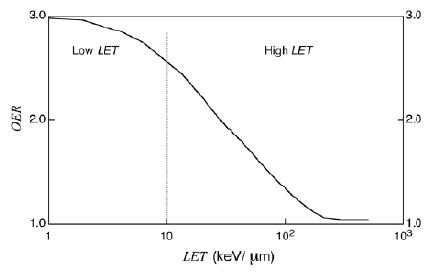
\includegraphics[width=8cm, keepaspectratio]{OER.png}
		\caption{Oxygen Enhancement Ratio in funzione del LET}
         \label{OER}
\end{figure}

\section{Strumenti di Dosimetria} 

I dosimetri possono essere attivi, se misurano la loro grandezza al variare del tempo, o passivi, se sono cumulativi. Un dosimetro utile ha le seguenti proprietà:
\begin{itemize}
\item Alta accuratezza e precisione
\item Segnale lineare su un range ampio
\item Poca dipendenza in questa linearità dalla dose, dal rate di dose e dall'energia della radiazione
\item Indipendenza dalla direzione della radiazione incidente
\item Alta risoluzione spaziale
\end{itemize}

Qualunque dosimetro perde linearità tra risposta e dose effettiva. Questo può avvenire per superlinearità o per saturazione. Il primo caso può anche essere utile avendo un software che si aspetta la superlinearità e la sfrutta per aumentare la risoluzione dello strumento.

Un esempio di dosimetro è la camera a ionizzazione. Di solito è cilindrica, delle dimensioni di una penna, con armatura esterna in grafite e interna in alluminio. Il segnale elettrico si può trasformare in una lettura di Exposure. Può anche essere a pozzo, per misurare grandezze relative a sorgenti puntiformi che si mettono sopra il pozzo. Questo tipo di camere ha alta sensibilità e può funzionare in maniera attiva.

Altro tipo di rivelatore è il Film Radiografico \cite{Films}, che consiste in un coating metallico che emette elettroni per effetto fotoelettrico quando è inciso da una radiazione, i quali vanno a ionizzare la sottostante emulsione di AgBr. A questo punto l'argento si neutralizza senza legarsi di nuovo col bromo. L'argento è nero, dunque quello che osservo quando la pellicola è sottoposta a radiazione è un annerimento graduale.
Infine si illumina la pellicola e ne si osserva l'opacità, stimabile come segue:

\begin{equation}
\text{OD}=\log_{10}\left(\frac{I}{I_0}\right)
\end{equation}

L'opacità è poi una funzione monotona dell'exposure, e dunque è possibile ricavare quest'ultima grandezza.

Un Film Radiocromico invece è una pellicola contenente una tinta che polimerizza quando viene investita da radiazione e dunque mostra colore dopo essere stata colpita (GafChromic).

Altro tipo di dosimetri sono quelli che si basano su fenomeni di luminescenza quali fosforescenza e fluorescenza \cite{TLD}. Attraverso il posizionamento di impurità si creano stati metastabili intermedi nel decadimento di elettroni eccitati dalla radiazione, che dunque passando per questi stati emettono luce visibile.

Infine vi sono i detector a semiconduttore in cui la radiazione ionizzante incidente crea coppie elettrone-lacuna che generano una corrente all'interno del semiconduttore.

Per quanto riguarda la dosimetria di neutroni si usano materiali che contengono nuclei ad alta sezione d'urto con i neutroni, così che la reazione crei particelle cariche, poi facilmente tracciabili. \\

Bibliografia e approfondimenti sulla dosimetria: \cite{Corvisiero2} \cite{Beringer3} \cite{Laitano}.
